\chapter{Specifikacija programske potpore}
		
	\section{Funkcionalni zahtjevi}

			
			\noindent \textbf{Dionici:}
			
			\begin{packed_enum}
				
				\item Administrator
				\item Korisnik/Posjetitelj				
				\item Organizator				
				\item Baza podataka
				\item PayPal
				\item Banka
				
				
			\end{packed_enum}
			
			\noindent \textbf{Aktori i njihovi funkcionalni zahtjevi:}
			
			
			\begin{packed_enum}
				\item  \underbar{Administrator (inicijator) može:}
				
				\begin{packed_enum}
					
					\item prijaviti se i odjaviti sa stranice
					\item pregledavati događaje
					\begin{packed_enum}
	
							\item  filtrirati događaje po vremenskom razdoblju
	
					\end{packed_enum}
					\item  upravljati korisnicima
					\begin{packed_enum}
						
							\item  urediti ili izbrisati korisničke profile
							\item  urediti ili izbrisati objave korisnika
																			
				    \end{packed_enum}
					\item  postavljati cijene članstva
					
				\end{packed_enum}
			
			 	\item  \underbar{Korisnik/Posjetitelj  (inicijator) može:}
			 	
			 	\begin{packed_enum}
			 		
			 		\item prijaviti se i odjaviti sa stranice
			 		\item napraviti profil
			 		\item prikazati profil i urediti ga
			 		\item pregledavati događaje
			 		\begin{packed_enum}
			 			
			 			\item  filtrirati događaje po vremenskom razdoblju i ostalim parametrima
			 			
			 		\end{packed_enum}
			 		
			 		\item uključiti obavijesti o najnovijim događajima po kriterijima: vrsta događanja i područje
			 		\item iskazati interese za događaj („sigurno dolazim“, „možda dolazim“, „ne dolazim“)
			 		\item recenzirati događaj
			 		
			 	\end{packed_enum}
			    
			    
			    \item  \underbar{Organizator (inicijator) može:}
				
				\begin{packed_enum}
					
					\item postaviti događaj
					\begin{packed_enum}
						
						\item  urediti ili izbrisati događaj
						\item  postaviti događaj sa plaćanjem ulaznice i platiti članarinu (Paypalom ili bankovnom karticom)
						
					\end{packed_enum}
					\item prijaviti se i odjaviti sa stranice
					\item napraviti profil
					\item prikazati profil i urediti ga
					\item pregledavati događaje
					\begin{packed_enum}
	
						\item filtrirati događaje po vremenskom razdoblju i ostalim parametrima
	
					\end{packed_enum}
					
				\end{packed_enum}
				
				
				\item  \underbar{Baza podataka (sudionik):}	
							
				\begin{packed_enum}				
				
					\item pohranjuje zapise o korisnicima i događajima
					\item pohranjuje iskazane interese za događaje
					\item pohranjuje recenzije događaja			
					\item pohranjuje informacije o cijenama članstva
					\item omogućuje prijavu i odjavu sa stranice (token)
				\end{packed_enum}

				\item  \underbar{PayPal (sudionik):}

				\begin{packed_enum}

				\item Odobrava transakcije potrebne za platiti članarinu

				\end{packed_enum}				
				
				\item  \underbar{Banka (sudionik):}				
				
				\begin{packed_enum}
						
				\item Odobrava transakcije potrebne za platiti članarinu 					
					
				\end{packed_enum}
			    
			   
					

												
			\end{packed_enum}
			
	
			\eject 
			
			
				
			\subsection{Obrasci uporabe}
							
					\noindent \underbar{\textbf{UC1 - Registracija posjetiteljskog računa}}
					\begin{packed_item}
					\item \textbf{Glavni sudionik:} Korisnik
					\item  \textbf{Cilj:} Izrada korisničkog računa za potrebe pregledavanja i posjećivanja događaja
					\item  \textbf{Sudionici:} Baza podataka
					\item  \textbf{Preduvjet:} -
					\item  \textbf{Opis osnovnog tijeka:}
					
					\item[] \begin{packed_enum}
						
						\item Korisnik izabire opciju registracije
						\item Korisnik unosi korisničke podatke koji se od njega traže
						\item Sustav provjerava ispravnost unesenih podataka
						\item Sustav šalje korisnika na prozor za prijavu na stranicu
					\end{packed_enum}
					
					\item  \textbf{Opis mogućih odstupanja:}
					
					\item[] \begin{packed_item}
						
						\item[2.a] Korisnik odabire već zauzeto korisničko ime ili e-mail
						\item[] \begin{packed_enum}
							
							\item Sustav obavještava korisnika o neuspješnoj registraciji i navodi razlog zašto
							registracija nije uspjela
							\item Korisnik mijenja potrebne podatke, završi registraciju ili odustane od registracije
							
						\end{packed_enum}
					\end{packed_item}

				\end{packed_item}
				
					\noindent \underbar{\textbf{UC2 - Registracija organizatorskog računa}}
					\begin{packed_item}
					\item \textbf{Glavni sudionik:} Korisnik
					\item  \textbf{Cilj:} Izrada korisničkog računa za potrebe stvaranja/organiziranja događaja
					\item  \textbf{Sudionici:} Baza podataka
					\item  \textbf{Preduvjet:} -
					\item  \textbf{Opis osnovnog tijeka:}
					
					\item[] \begin{packed_enum}
						
						\item Korisnik izabire opciju registracije uz odabir polja "Organizator"
						\item Korisnik unosi korisničke podatke koji se od njega traže
						\item Sustav provjerava ispravnost unesenih podataka
						\item Sustav šalje korisnika na prozor za prijavu na stranicu
					\end{packed_enum}
					
							\item  \textbf{Opis mogućih odstupanja:}
					
					\item[] \begin{packed_item}
						
						\item[2.a] Korisnik odabire već zauzeto korisničko ime ili e-mail 
						\item[] \begin{packed_enum}
							
							\item Sustav obavještava korisnika o neuspješnoj registraciji i navodi razlog zašto
							registracija nije uspjela 
							\item Korisnik mijenja potrebne podatke, završi registraciju ili odustane od registracije
							
						\end{packed_enum}
					\end{packed_item}
					
				\end{packed_item}
			
					\noindent \underbar{\textbf{UC3 - Prijava na stranicu}}
					\begin{packed_item}
				
				\item \textbf{Glavni sudionik: } Korisnik, Administrator
				\item  \textbf{Cilj:} Dobiti pristup stranici
				\item  \textbf{Sudionici:} Baza podataka
				\item  \textbf{Preduvjet:} Korisnik ima registrirani račun ili ima račun s pravima administratora
				\item  \textbf{Opis osnovnog tijeka:}
				
				\item[] \begin{packed_enum}
					
					\item Korisnik/Administrator otvara stranicu
					\item Korisnik/Administrator unosi korisničke podatke za prijavu na stranicu
					\item Sustav prepoznaje je li prijavljeni račun korisnički ili administratorski te otvara odgovarajuću početnu stranicu
				\end{packed_enum}
				
				\item  \textbf{Opis mogućih odstupanja:}
				
				\item[] \begin{packed_item}
					
					\item[2.a] Korisnik unosi pogrešnu kombinaciju imena i lozinke za prijavu
					\item[] \begin{packed_enum}
						
						\item Sustav javlja korisniku da je prijava neuspješna, nudi ponovnu prijavu ili stvaranje
						novog korisničkog računa
					\end{packed_enum}
					
					
				\end{packed_item}
			\end{packed_item}
			
				
					\noindent \underbar{\textbf{UC4 - Pregled događaja}}
					\begin{packed_item}
					\item \textbf{Glavni sudionik:} Korisnik
					\item  \textbf{Cilj:} Pregledati dostupne događaje
					\item  \textbf{Sudionici:} Baza podataka
					\item  \textbf{Preduvjet:} Korisnik se prijavio na stranicu
					\item  \textbf{Opis osnovnog tijeka:}
					
					\item[] \begin{packed_enum}
						
						\item Nakon prijave korisnika se prebacuje na stranicu za pregledavanje događaja - "Svi događaji"
						\item Korisniku su događaji izlistani jedan ispod drugog
						\item Kod svakog događaja prikazane su sve informacije o događaju (npr. datum održavanja, broj zainteresiranih itd.) te pripadajuća fotografija
					\end{packed_enum}
					
				\end{packed_item}
				
					\noindent \underbar{\textbf{UC5 - Filtriranje događaja}}
					\begin{packed_item}
					\item \textbf{Glavni sudionik:} Korisnik
					\item  \textbf{Cilj:} Pregledati događaje prema željenim kriterijima
					\item  \textbf{Sudionici:} Baza podataka
					\item  \textbf{Preduvjet:} Korisnik je prijavljen i nalazi se na stranici za pregled događaja
					\item  \textbf{Opis osnovnog tijeka:}
					
					\item[] \begin{packed_enum}
						
						\item Korisnik na stranici za pregledavanje događaja bira između više ponuđenih opcija za filtriranje događaja
					\end{packed_enum}
					
					\item  \textbf{Opis mogućih odstupanja:}
					
					\item[] \begin{packed_item}
						
						\item[1.a] Ne postoji događaj koji odgovara korisnikovoj kombinaciji filtera
						\item[] \begin{packed_enum}
							
							\item Sustav korisniku prikazuje stranicu bez događaja
							
						\end{packed_enum}
					\end{packed_item}
				\end{packed_item}

					\noindent \underbar{\textbf{UC6 - Prikazivanje osobnog profila}}
					\begin{packed_item}
					\item \textbf{Glavni sudionik:} Korisnik 
				\item  \textbf{Cilj:} Pregledati osobni profil
				\item  \textbf{Sudionici:} Baza podataka
				\item  \textbf{Preduvjet:} Korisnik je prijavljen na stranici
				\item  \textbf{Opis osnovnog tijeka:}
	
				\item[] \begin{packed_enum}
		
				\item Korisnik klikne na ime svog računa te odabire opciju "Profil"
				\item Sustav prikazuje stranicu korisnikovog osobnog profila
				\end{packed_enum}
	
			\end{packed_item}

					\noindent \underbar{\textbf{UC7 - Uređivanje profila}}
					\begin{packed_item}
	\item \textbf{Glavni sudionik:} Korisnik
	\item  \textbf{Cilj:} Izmjena osobnih podataka
	\item  \textbf{Sudionici:} Baza podataka
	\item  \textbf{Preduvjet:} Korisnik je prijavljen na stranici i odabrao je opciju "Profil" (UC6)
	\item  \textbf{Opis osnovnog tijeka:}
	
	\item[] \begin{packed_enum}
		
		\item Korisnik na stranici osobnog profila pored podatka koji želi promijeniti pritisne ikonu olovke
		\item Sustav omogućuje izmjenu podatka
		\item Korisnik mijenja podatak
		\item Korisnik odabire ikonu kvačice
		\item Korisnik odabire opciju "SPREMI"
		\item Sustav korisniku javlja da su promjene uspješno pohranjene
	\end{packed_enum}
	
	\item  \textbf{Opis mogućih odstupanja:}
	
	\item[] \begin{packed_item}
		
		\item[4.a] Korisnik je promijenio korisničko ime ili e-mail u nešto što već postoji u sustavu
		\item[] \begin{packed_enum}
			
			\item Sustav javlja korisniku da je došlo do pogreške
			\item Korisnik ponovno upisuje ime/e-mail ili odustaje od promjena te ih briše pritiskom na ikonu križića
			
		\end{packed_enum}
	\end{packed_item}
\end{packed_item}

					\noindent \underbar{\textbf{UC8 - Odjava sa stranice}}
					\begin{packed_item}
	\item \textbf{Glavni sudionik:} Korisnik, Administrator
	\item  \textbf{Cilj:} Odjaviti se sa stranice
	\item  \textbf{Sudionici:} Baza podataka
	\item  \textbf{Preduvjet:} Korisnik/Administrator je prijavljen na stranici
	\item  \textbf{Opis osnovnog tijeka:}
	
	\item[] \begin{packed_enum}
		
		\item Korisnik/Administrator nakon klika na korisničko ime odabire opciju "Odjava"
		\item Sustav odjavljuje korisnika/administratora sa stranice
	\end{packed_enum}

\end{packed_item}

					\noindent \underbar{\textbf{UC9 - Izražavanje interesa}}
\begin{packed_item}
	\item \textbf{Glavni sudionik:} Posjetitelj
	\item  \textbf{Cilj:} Izraziti interes za neki ponuđeni događaj
	\item  \textbf{Sudionici:} Baza podataka
	\item  \textbf{Preduvjet:} Korisnik je prijavljen na stranici i njegov račun je posjetiteljski
	\item  \textbf{Opis osnovnog tijeka:} 
	
	\item[] \begin{packed_enum}
		
		\item Posjetitelj pregledava događaje (UC4) te dolazi do događaja koji ga zanima
		\item Posjetitelj odabire jednu od tri ponuđene opcije interesa: "DOLAZIM", "MOŽDA", "NE DOLAZIM"
		\item Sustav pohranjuje podatak o posjetiteljevom interesu, a u slučaju da je posjetitelj odabrao "DOLAZIM" ili "MOŽDA", ažurira odgovarajući brojač kod prikaza događaja te dodaje taj događaj na popis posjetiteljevih interesnih događaja
	\end{packed_enum}
	
		\item  \textbf{Opis mogućih odstupanja:}
	
	\item[] \begin{packed_item}
		
		\item[2.a] Posjetitelj odabrao pogrešnu opciju ili želi promijeniti interes
		\item[] \begin{packed_enum}
			
			\item Posjetitelj odabire neku drugu ponuđenu opciju
			
		\end{packed_enum}
		
	\end{packed_item}

\end{packed_item}


					\noindent \underbar{\textbf{UC10 - Pregled posjetiteljevih interesnih događaja}}
\begin{packed_item}
	\item \textbf{Glavni sudionik:} Posjetitelj
	\item  \textbf{Cilj:} Pregledati sve događaje koje posjetitelja zanimaju
	\item  \textbf{Sudionici:} Baza podataka
	\item  \textbf{Preduvjet:} Posjetitelj je prijavljen i na početnoj je stranici
	\item  \textbf{Opis osnovnog tijeka:}
	
	\item[] \begin{packed_enum}
		
		\item Posjetitelj na početnoj stranici odabire opciju "MOJI DOGAĐAJI"
		\item Sustav posjetitelju otvara stranicu na kojoj je popis svih događaja za koje je postavio interes "DOLAZIM" ili "MOŽDA"
	\end{packed_enum}
	
	\item  \textbf{Opis mogućih odstupanja:}
	
	\item[] \begin{packed_item}
		
		\item[2.a] Posjetitelj nije odabrao odgovarajuću opciju niti za jedan događaj
		\item[] \begin{packed_enum}
			
			\item Sustav korisniku prikazuje stranicu bez događaja
			
		\end{packed_enum}
	\end{packed_item}
\end{packed_item}

					\noindent \underbar{\textbf{UC11 - Recenziranje događaja}}
\begin{packed_item}
	\item \textbf{Glavni sudionik:} Posjetitelj
	\item  \textbf{Cilj:} Ostaviti recenziju na posjećen događaj
	\item  \textbf{Sudionici:} Baza podataka
	\item  \textbf{Preduvjet:} Posjetitelj je prijavljen na stranicu i nalazi se na stranici pregleda interesnih događaja (UC10)
	\item  \textbf{Opis osnovnog tijeka:}
	
	\item[] \begin{packed_enum}
		
		\item Posjetitelj dolazi do događaja kojeg želi recenzirati
		\item Ako je događaj završio i nije prošlo 48 sati od njegovog završetka, posjetitelju je otvoren obrazac za recenziranje u kojem može odabrati ocjenu te napisati recenziju
		\item Posjetitelj završava recenziju i odabire opciju "Pohrani recenziju"
		\item Sustav pohranjuje recenziju
		\item Ako događaj nije završio, ili je prošlo više od 48 sati od njegovog završetka, posjetitelju nije otvoren obrazac za recenziranje

	\end{packed_enum}
	
			\item  \textbf{Opis mogućih odstupanja:}
			
	\item[] \begin{packed_item}
		\item[2.a] Posjetitelj napisao opis recenzije, no nije izabrao ocjenu
			\item[] \begin{packed_enum}
		\item Sustav ne dozvoljava pohranjivanje recenzije dok ocjena nije odabrana
		\item Posjetitelj odabire ocjenu i pohranjuje recenziju, ili odustaje
		
	\end{packed_enum}
\end{packed_item}
\end{packed_item}

					\noindent \underbar{\textbf{UC12 - Automatsko slanje obavijesti}}
\begin{packed_item}
	\item \textbf{Glavni sudionik:} Posjetitelj
	\item  \textbf{Cilj:} Kroz aplikaciju postaviti automatsko primanje obavijesti za najnovije događaje na temelju zadanih kriterija
	\item  \textbf{Sudionici:} Baza podataka
	\item  \textbf{Preduvjet:} Posjetitelj prijavljen i nalazi se na stranici osobnog korisničkog računa
	\item  \textbf{Opis osnovnog tijeka:}
	
	\item[] \begin{packed_enum}
		
		\item Korisnik ispod naznake "Pretplate na obavijesti" zadaje kriterij notifikacija - vrstu događaja te lokaciju
		\item Korisnik sprema pretplatu na obavijesti pritiskom na ikonu plusa te sustav pohranjuje korisnikov odabir
	\end{packed_enum}
	
	
	\item  \textbf{Opis mogućih odstupanja:}
		\item[] \begin{packed_item}
	\item[2.a] Korisnik odabrao pretplatu na obavijesti, ali se predomislio i ne želi je
	\item[] \begin{packed_enum}
		
		\item Sustav omogućuje korisniku brisanje pretplate klikom na ikonu koša za smeće
		
	\end{packed_enum}
\end{packed_item}
\end{packed_item}

					\noindent \underbar{\textbf{UC13 - Postavljanje događaja}}
\begin{packed_item}
	\item \textbf{Glavni sudionik:} Organizator
	\item  \textbf{Cilj:} Postaviti novi događaj
	\item  \textbf{Sudionici:} Baza podataka
	\item  \textbf{Preduvjet:} Korisnik je prijavljen na stranici i ima organizatorski račun
	\item  \textbf{Opis osnovnog tijeka:}
	
	\item[] \begin{packed_enum}
		
		\item Organizator započinje proces izrade novog događaja pritiskom na ikonu plusa u desnom donjem kutu
		\item Organizatoru se otvara obrazac za dodavanje događaja
		\item Organizator popunjava sve potrebne podatke o događaju te postavlja događaj odabirom opcije "DODAJ"
		\item Sustav pohranjuje novi događaj te vraća organizatora na stranicu "Moji događaji"
	\end{packed_enum}
	
	\item  \textbf{Opis mogućih odstupanja:}
	
	\item[] \begin{packed_item}
		
		\item[4.a] Organizator odustaje od objave događaja
		\item[] \begin{packed_enum}
			
			\item Organizator ima opciju "Odustani" čijim odabirom prekida proces stvaranja novog događaja
			
		\end{packed_enum}
	\end{packed_item}
\end{packed_item}

					\noindent \underbar{\textbf{UC14 - Postavljanje događaja sa plaćanjem ulaznice}}
\begin{packed_item}
	\item \textbf{Glavni sudionik:} Organizator
	\item  \textbf{Cilj:} Postaviti događaj na kojem će biti naplaćivanje ulaznica
	\item  \textbf{Sudionici:} Baza podataka
	\item  \textbf{Preduvjet:} Korisnik prijavljen na stranicu, ima organizatorski korisnički račun i plaćenu pretplatu
	\item  \textbf{Opis osnovnog tijeka:}
	
	\item[] \begin{packed_enum}
		
		\item Organizator pri ispunjavanju podataka o događaju kojeg želi postaviti stavlja željenu cijenu događaja (veću od 0) 
		\item  Organizator odabire opciju "DODAJ", sustav pohranjuje novi događaj te vraća organizatora na stranicu "Moji događaji"
	\end{packed_enum}
	
	\item  \textbf{Opis mogućih odstupanja:}
	
	\item[] \begin{packed_item}
		
		\item[2.a] Organizator nema plaćenu članarinu
		\item[] \begin{packed_enum}
			
			\item Sustav javlja organizatoru kako nema plaćenu članarinu i ne objavljuje događaj
			
		\end{packed_enum}

	\end{packed_item}
\end{packed_item}


					\noindent \underbar{\textbf{UC15 - Plaćanje članarine}}
\begin{packed_item}
	\item \textbf{Glavni sudionik:} Organizator
	\item  \textbf{Cilj:} Platiti članarinu kako bi se mogao postaviti događaj na kojem će se naplaćivati ulaznice
	\item  \textbf{Sudionici:} Baza podataka, PayPal, Banka
	\item  \textbf{Preduvjet:} Organizator se nalazi na stranici osobnog korisničkog računa
	\item  \textbf{Opis osnovnog tijeka:}
	
	\item[] \begin{packed_enum}
		\item Organizator odabire opciju "PRETPLATA"
		\item Organizator odabire način plaćanja članarine - plaćanje PayPal-om ili plaćanje bankovnom karticom, ispunjava podatke i odabire opciju "Pretplati se"
		\item Sustav javlja organizatoru da je plaćanje članarine uspješno
	\end{packed_enum}
	
		\item  \textbf{Opis mogućih odstupanja:}
	
	\item[] \begin{packed_item}
		
		\item[2.a] Transakcija je neuspješna
		\item[] \begin{packed_enum}
			
			\item Sustav javlja organizatoru kako transakcija nije prošla
			\item Organizator ponavlja postupak ili odustaje od plaćanja odabirom opcije "Povratak na profil"
			
		\end{packed_enum}
		
	\end{packed_item}
	
\end{packed_item}

					\noindent \underbar{\textbf{UC16 - Pregled vlastitih događaja}}
\begin{packed_item}
	\item \textbf{Glavni sudionik:} Organizator
	\item  \textbf{Cilj:} Pregledati vlastite postavljene događaje 
	\item  \textbf{Sudionici:} Baza podataka
	\item  \textbf{Preduvjet:} Organizator prijavljen na stranicu
	\item  \textbf{Opis osnovnog tijeka:}
	
	\item[] \begin{packed_enum}
		
		\item Organizator na početnoj stranici odabire opciju "MOJI DOGAĐAJI"
		\item Sustav otvara organizatoru stranicu na kojoj prikazuje sve njegove postavljene događaje
	\end{packed_enum}
	
	\item  \textbf{Opis mogućih odstupanja:}
	
	\item[] \begin{packed_item}
		
		\item[2.a] Organizator nema niti jedan postavljen događaj
		\item[] \begin{packed_enum}
			
			\item Sustav korisniku prikazuje stranicu bez događaja
			
		\end{packed_enum}
	\end{packed_item}
\end{packed_item}

					\noindent \underbar{\textbf{UC17 - Uređivanje/brisanje događaja}}
\begin{packed_item}
	\item \textbf{Glavni sudionik:} Organizator
	\item  \textbf{Cilj:} Urediti ili obrisati postavljeni događaj
	\item  \textbf{Sudionici:} Baza podataka
	\item  \textbf{Preduvjet:} Organizator prijavljen, nalazi se na stranici "MOJI DOGAĐAJI" te ima postavljeni događaj
	\item  \textbf{Opis osnovnog tijeka:}
	
	\item[] \begin{packed_enum}
		
		\item Organizator pronalazi događaj kojeg želi urediti ili izbrisati i pritisne na ikonu olovke, odnosno koša za smeće
		\item Ako je izabrana ikona olovke, sustav otvara organizatoru obrazac za postavljanje događaja ispunjen s njegovim podacima i dozvoljava uređivanje; organizator zatim uređuje podatke i bira opciju "Spremi"
		\item Ako je izabrana ikona koša za smeće, sustav briše događaj iz baze podataka
	\end{packed_enum}
	
	\item  \textbf{Opis mogućih odstupanja:}
	
	\item[] \begin{packed_item}
		
		\item[2.a] Organizator greškom unio krive podatke
		\item[] \begin{packed_enum}
			
			\item Sustav dozvoljava izmjenu podataka neograničen broj puta
			
		\end{packed_enum}
	\end{packed_item}
\end{packed_item}



\noindent \underbar{\textbf{UC18 - Administrativni pregled događaja}}
\begin{packed_item}
	\item \textbf{Glavni sudionik:} Administrator
	\item  \textbf{Cilj:} Pregledati događaje kao administrator
	\item  \textbf{Sudionici:} Baza podataka
	\item  \textbf{Preduvjet:} Korisnik je registriran, ima prava administratora i uspješno se prijavio
	\item  \textbf{Opis osnovnog tijeka:}
	
	\item[] \begin{packed_enum}
		
		\item Administrator na početnoj stranici odabire opciju "SVI DOGAĐAJI"
		\item Sustav administratora prebacuje na stranicu s popisom događaja
	\end{packed_enum}
	
\end{packed_item}


\noindent \underbar{\textbf{UC19 - Postavljanje cijene pretplate}}
\begin{packed_item}
	\item \textbf{Glavni sudionik:} Administrator
	\item  \textbf{Cilj:} Postaviti ili promijeniti cijenu pretplate 
	\item  \textbf{Sudionici:} Baza podataka
	\item  \textbf{Preduvjet:} Korisnik je registriran, ima prava administratora i nalazi se na stranici osobnog profila
	\item  \textbf{Opis osnovnog tijeka:}
	
	\item[] \begin{packed_enum}
		
		\item Administrator ispod naznake "Cijena pretplate" ažurira cijenu pretplate i odabire opciju "Spremi"

	\end{packed_enum}
	
\end{packed_item}


\noindent \underbar{\textbf{UC20 - Upravljanje korisnicima}}
\begin{packed_item}
	\item \textbf{Glavni sudionik:} Administrator
	\item  \textbf{Cilj:} Pregledati korisničke račune i/ili njihove objave
	\item  \textbf{Sudionici:} Baza podataka
	\item  \textbf{Preduvjet:} Korisnik je registriran i ima prava administratora
	\item  \textbf{Opis osnovnog tijeka:}
	
	\item[] \begin{packed_enum}
		
		\item Administrator na početnoj stranici odabire opciju "SVI KORISNICI"
		\item Sustav administratora prebacuje na stranicu s popisom korisnika i njihovim podacima

	\end{packed_enum}

\end{packed_item}


\noindent \underbar{\textbf{UC21 - Uređivanje/brisanje korisnika}}
\begin{packed_item}
	\item \textbf{Glavni sudionik:} Administrator
	\item  \textbf{Cilj:} Urediti ili obrisati korisnika
	\item  \textbf{Sudionici:} Baza podataka
	\item  \textbf{Preduvjet:} Korisnik je registriran i ima prava administratora
	\item  \textbf{Opis osnovnog tijeka:}
	
	\item[] \begin{packed_enum}
		
		\item Administrator pronalazi željenog korisnika
		\item Administrator odabire ikonu koša za smeće te briše njegove podatke iz baze podataka
	\end{packed_enum}

\end{packed_item}


\noindent \underbar{\textbf{UC22 - Uređivanje/brisanje objava korisnika}}
\begin{packed_item}
	\item \textbf{Glavni sudionik:} Administrator
	\item  \textbf{Cilj:} Urediti/obrisati objave korisnika
	\item  \textbf{Sudionici:} Baza podataka
	\item  \textbf{Preduvjet:} Korisnik je registriran, ima prava administratora i pregledava sve događaje
	\item  \textbf{Opis osnovnog tijeka:}
	
	\item[] \begin{packed_enum}
		
		\item Administrator pronalazi događaj kojeg želi urediti ili izbrisati te pritisne opciju na ikonu olovke ili ikonu koša za smeće
		\item Ako je odabrana ikona olovke, sustav otvara obrazac za postavljanje događaja ispunjen s njegovim podacima i dozvoljava uređivanje; administrator zatim uređuje podatke i bira opciju "Spremi"
		\item Ako je izabrana ikona koša za smeće, sustav briše događaj iz baze podataka
	\end{packed_enum}
	
\end{packed_item}



					
				\subsubsection{Dijagrami obrazaca uporabe}
					
					\begin{figure}[H]
						\includegraphics[scale=0.35]{dijagrami/Opći_UC_dijagram_v2.0.png} %veličina slike u odnosu na originalnu datoteku i pozicija slike
						\centering
						\caption{Dijagram obrasca uporabe, opća funkcionalnost aktora}
						\label{fig:promjene}
					\end{figure}
					
					\begin{figure}[H]
						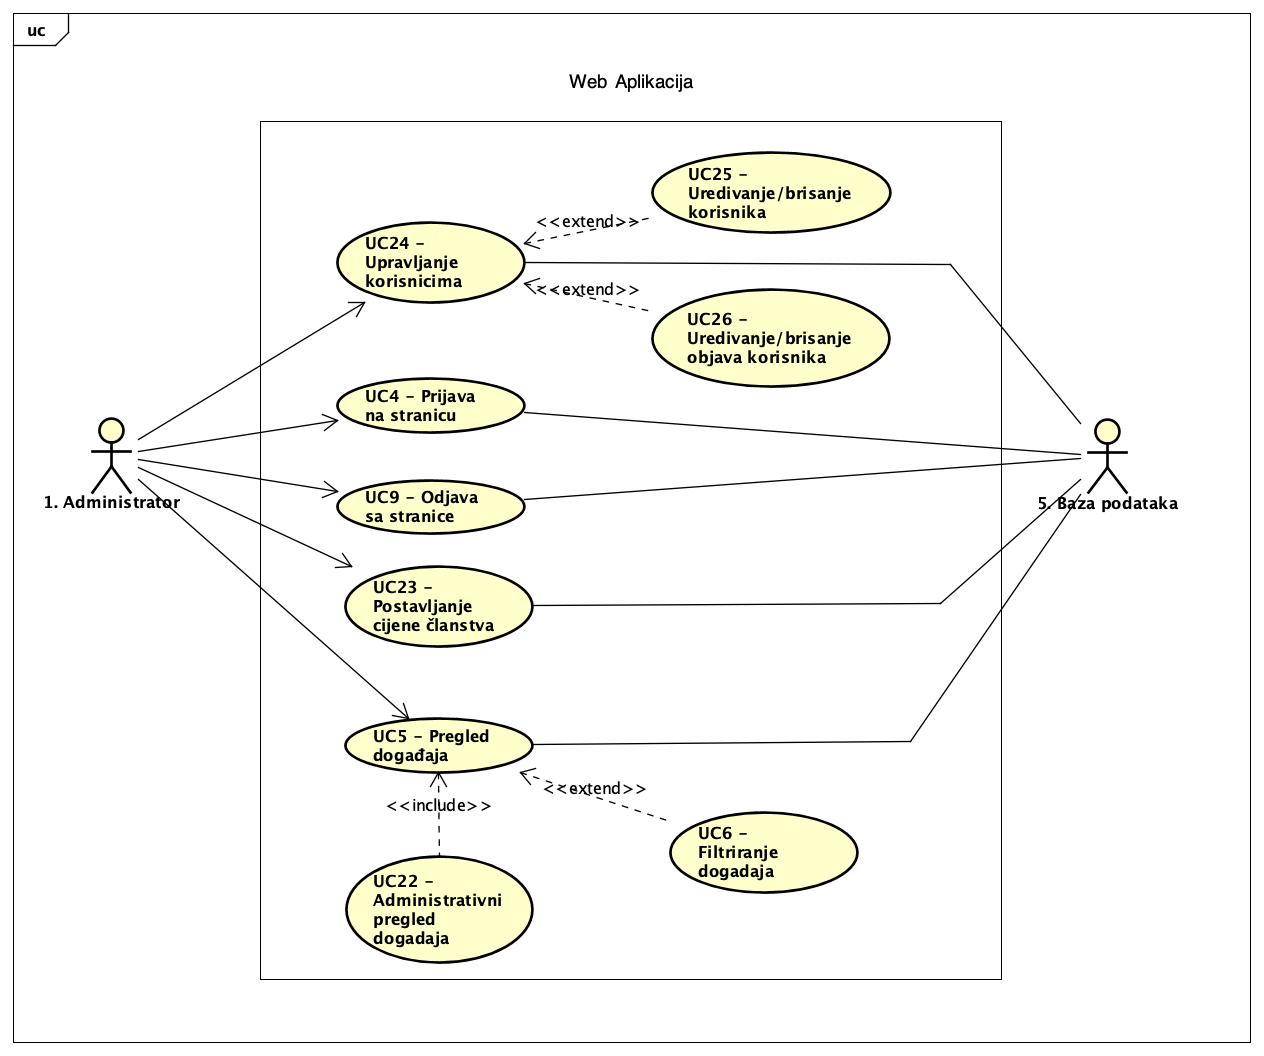
\includegraphics[scale=0.5]{dijagrami/Administrator_UC_dijagram.png} %veličina slike u odnosu na originalnu datoteku i pozicija slike
						\centering
						\caption{Dijagram obrasca uporabe, funkcionalnost administratora}
						\label{fig:promjene}
					\end{figure}
					
					\begin{figure}[H]
						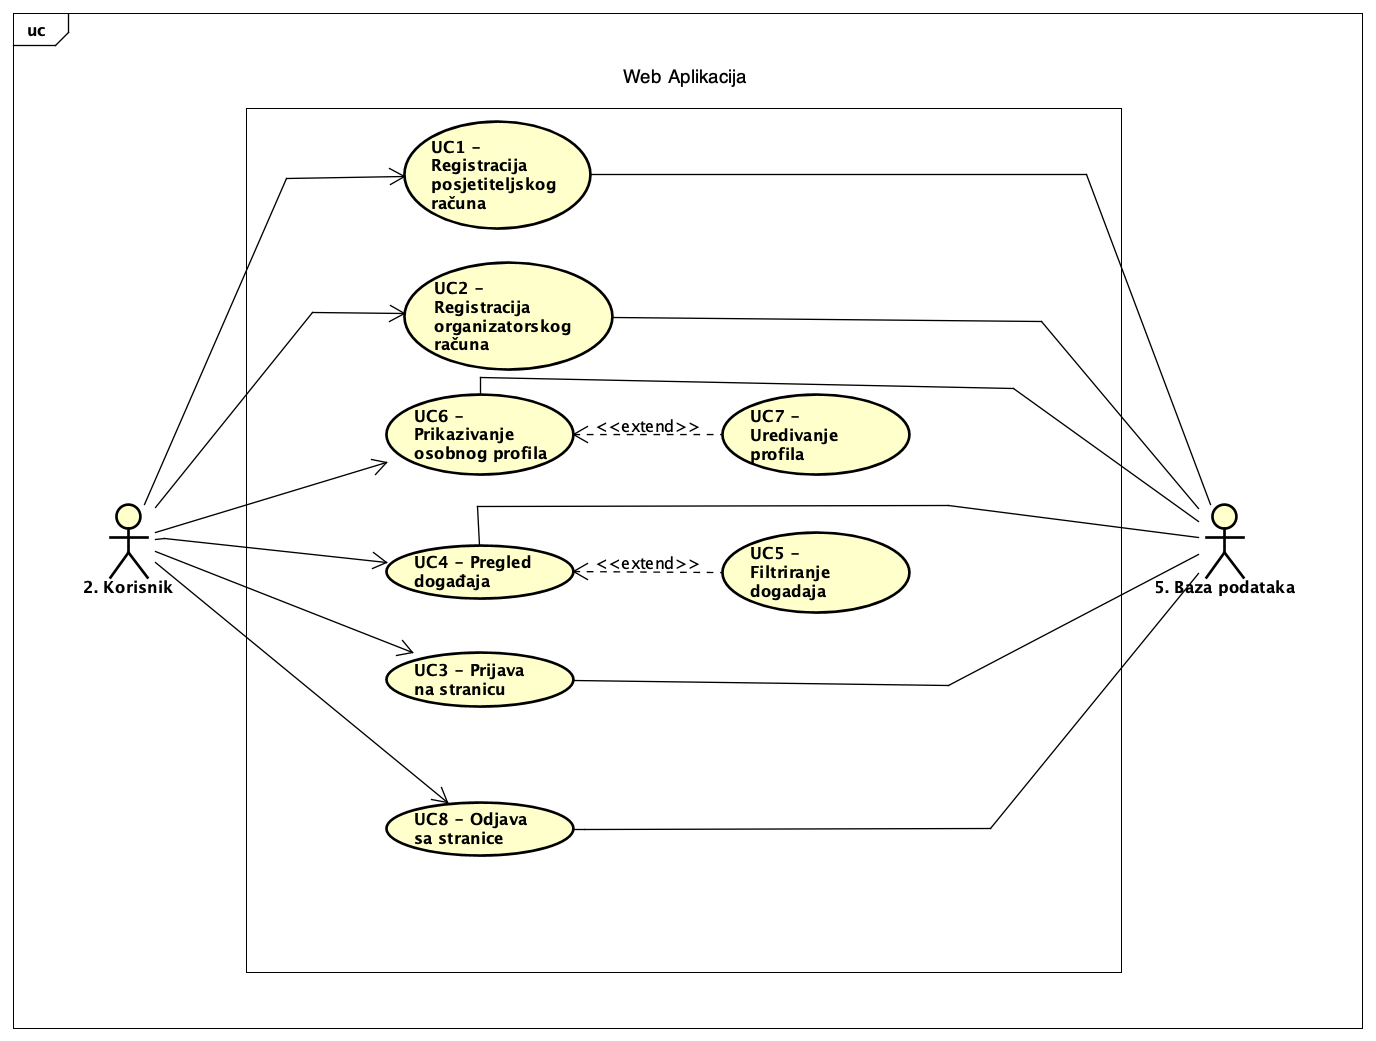
\includegraphics[scale=0.5]{dijagrami/Korisnik_UC_dijagram.png} %veličina slike u odnosu na originalnu datoteku i pozicija slike
						\centering
						\caption{Dijagram obrasca uporabe, funkcionalnost korisnika}
						\label{fig:promjene}
					\end{figure}
					
					\begin{figure}[H]
						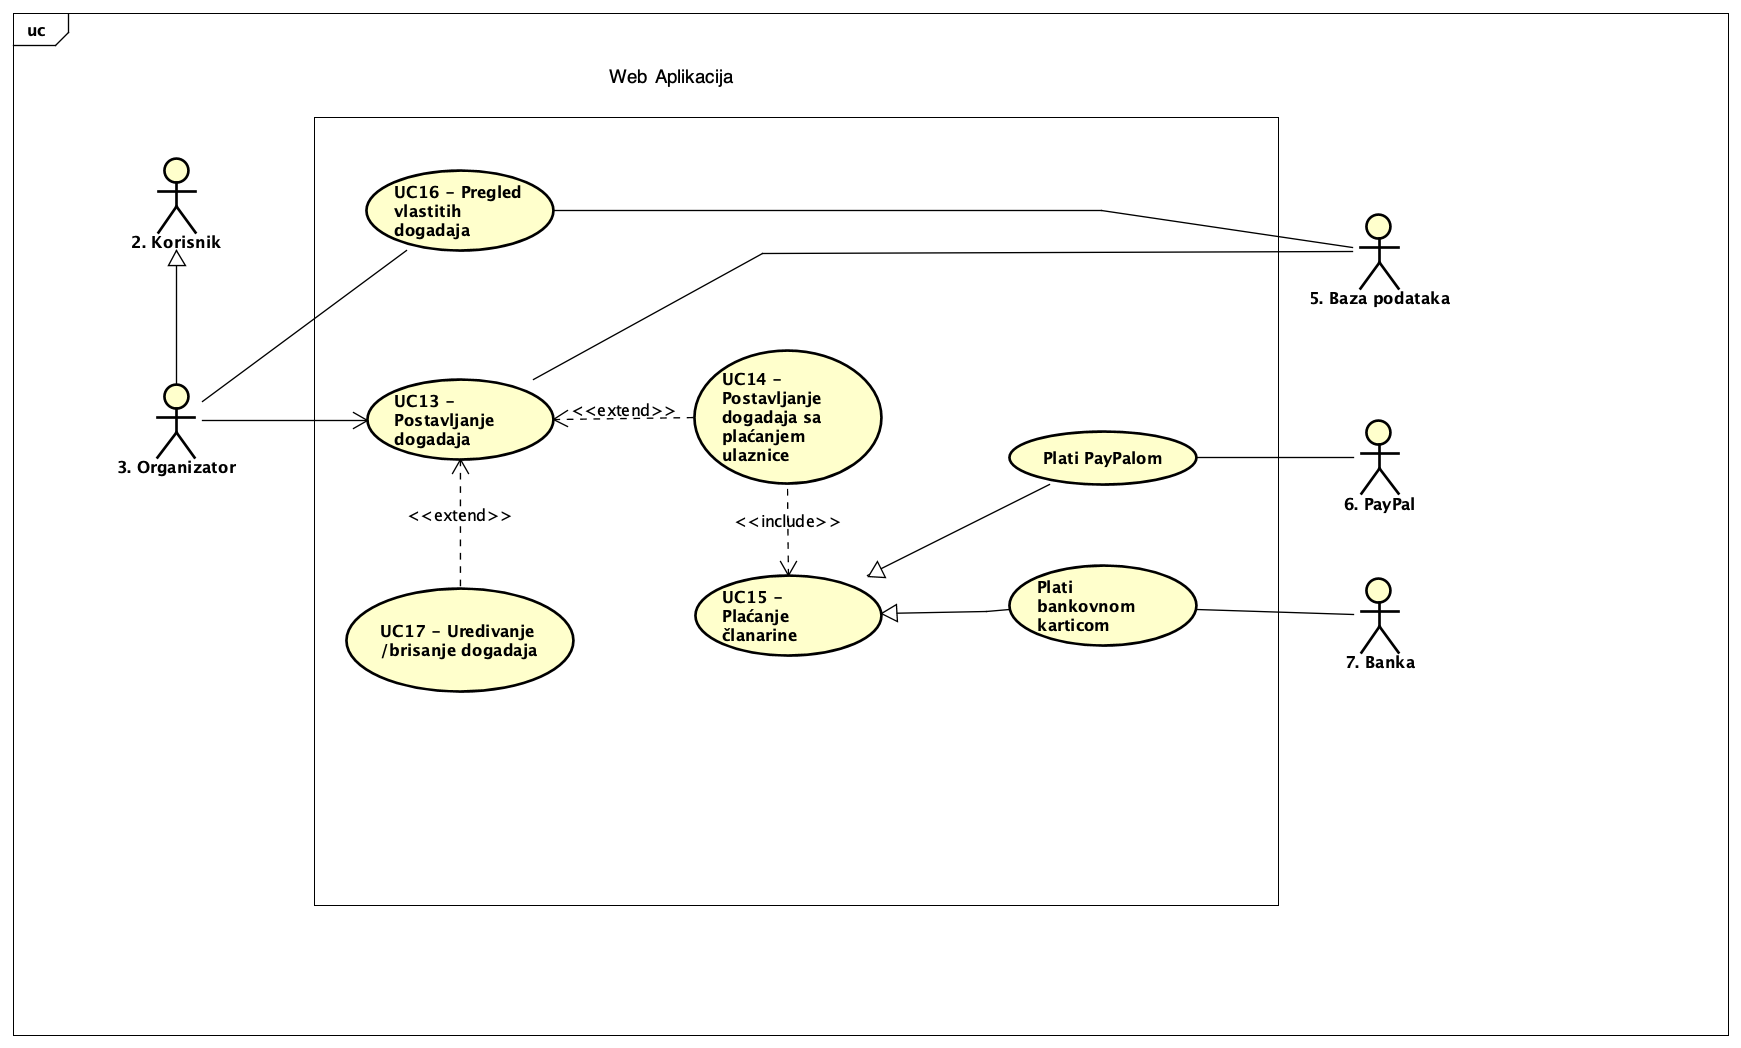
\includegraphics[scale=0.37]{dijagrami/Organizator_UC_dijagram.png} %veličina slike u odnosu na originalnu datoteku i pozicija slike
						\centering
						\caption{Dijagram obrasca uporabe, funkcionalnost organizatora}
						\label{fig:promjene}
					\end{figure}
					
					\begin{figure}[H]
						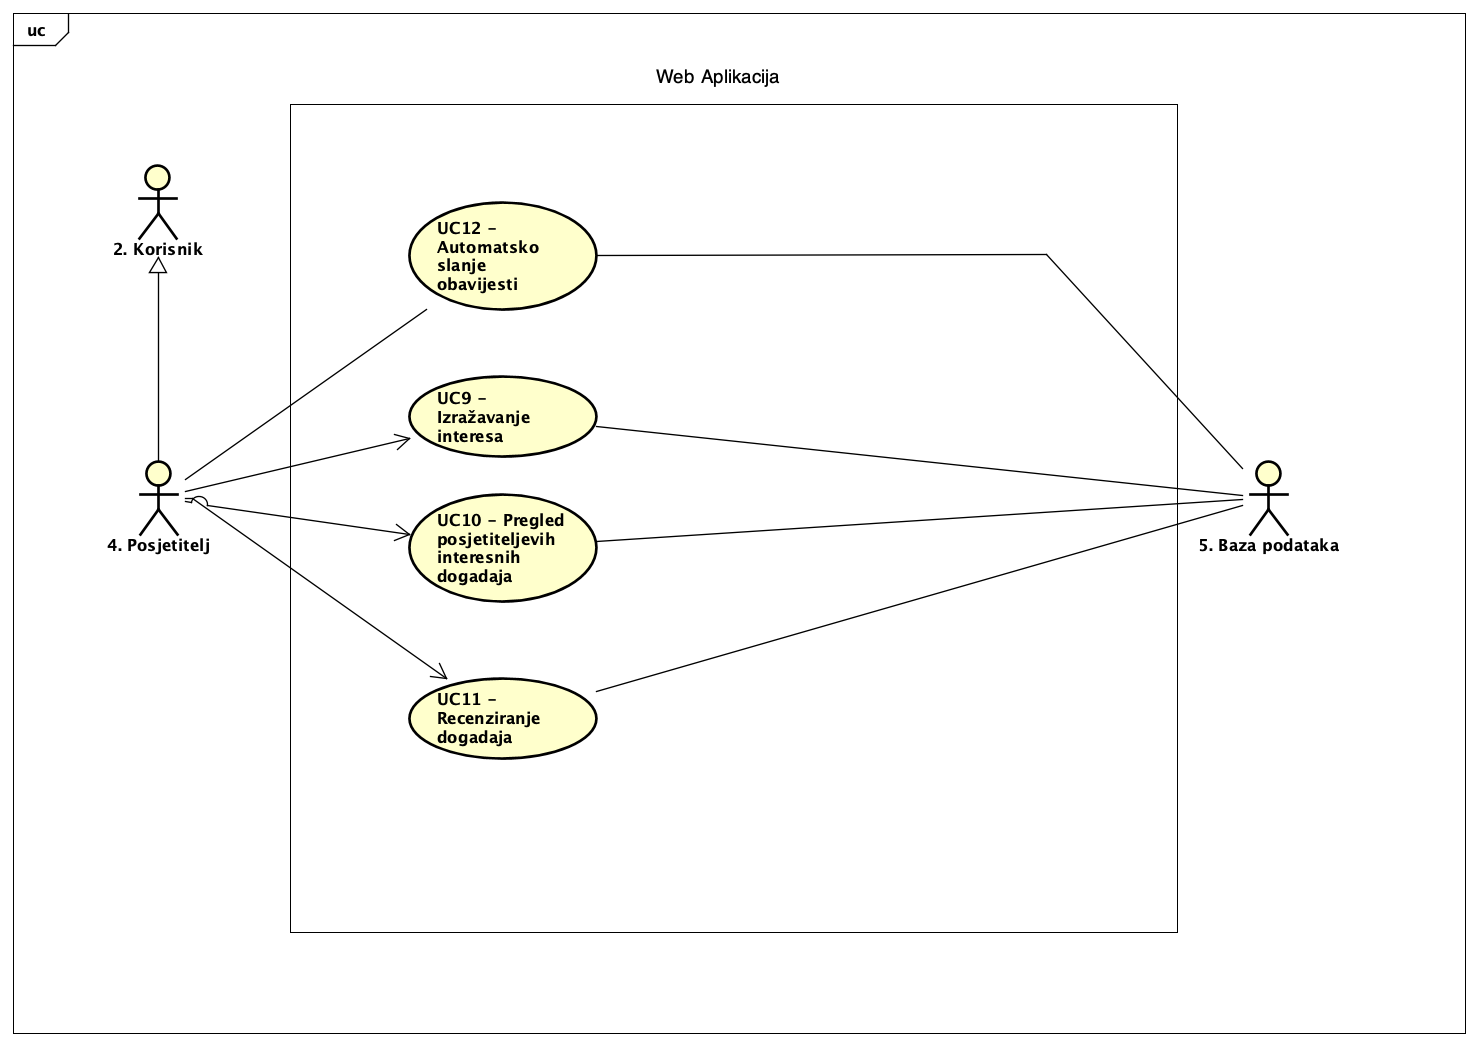
\includegraphics[scale=0.42]{dijagrami/Posjetitelj_UC_dijagram.png} %veličina slike u odnosu na originalnu datoteku i pozicija slike
						\centering
						\caption{Dijagram obrasca uporabe, funkcionalnost posjetitelja}
						\label{fig:promjene}
					\end{figure}
					
				
				\eject		
				
			\subsection{Sekvencijski dijagrami}
				
	
				\textbf{\large {Obrazac uporabe UC1 - Registracija}}
				\newline
				\normalsize
				Korisnik prilikom procesa registracije odabire opciju registracije: Posjetitelj ili Organizator. Na temelju odabira, korisnik dohvaća obrazac za registraciju. Nakon ispunjavanja obrasca, korisnik šalje zahtjev za registraciju. Nakon provjere ispravnosti unesenih podataka moguće su dvije opcije:
				
				\begin{packed_item}
					\item {Podaci ispravni:} u slučaju ispravnih podataka vrši se spremanje korisničkih podataka te korisnik prima poruku "Registracija uspješna" te slijedi prikaz za prijavu
					\item {Podaci neispravni:} Korisnik prima poruku da su podaci neispravni te može unijeti podatke ispočetka
				\end{packed_item}
				
				\begin{figure}[H]
					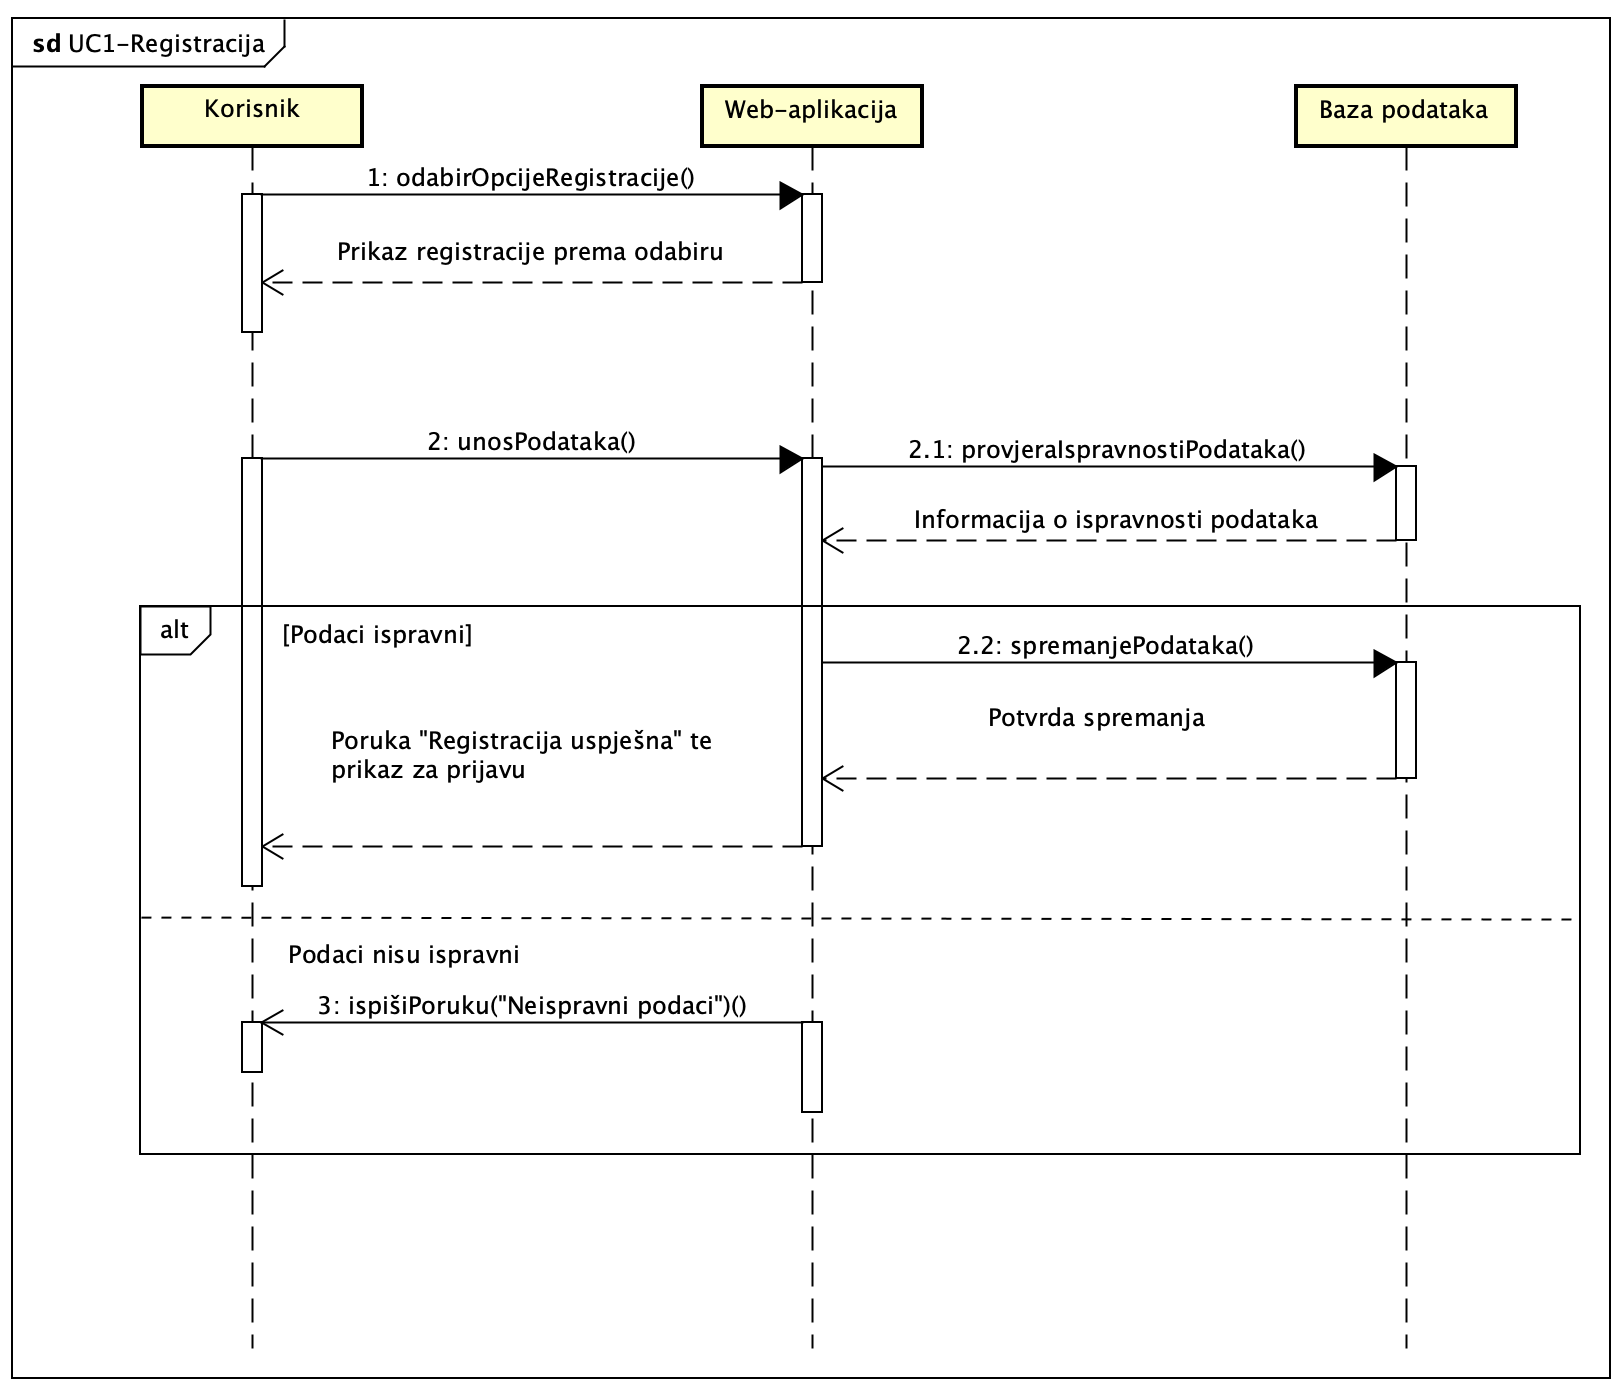
\includegraphics[scale=0.5]{dijagrami/sd-UC1-Registracija.png} %veličina slike u odnosu na originalnu datoteku i pozicija slike
					\centering
					\caption{Sekvencijski dijagram za UC1}
					\label{fig:promjene}
				\end{figure}
				\eject		
				
				\textbf{\large {Obrazac uporabe UC16 - Postavljanje događaja}}
				\newline
				\normalsize
				Tijekom procesa postavljanja događaja Organizator ima mogućnost izabrati objavu bez plaćanje ulaznice za događaj ili uz plaćanje. U slučaju postavljanja događaja bez plaćanja ulaznice odmah dohvaća obrazac za novi događaj. 
				Nakon slanja popunjenog obrasca sa svim potrebnim informacija, Organizator zaprima potvrdu za postavljanje događaja te ima mogućnost potvrditi ili odustati od objave. Ukoliko dođe do potvrde, informacije o događaju se spremaju te se isti objavljuje, u suprotnom Organizator dobiva potvrdu odustajanja.
				
				\begin{figure}[H]
					\includegraphics[scale=0.5]{dijagrami/sd-UC16-Postavljanje-događaja.png} %veličina slike u odnosu na originalnu datoteku i pozicija slike
					\centering
					\caption{Sekvencijski dijagram za UC16}
					\label{fig:promjene}
				\end{figure}
				\eject		
				
				\textbf {\large {Obrazac uporabe UC19 - Plaćanje članarine}}
				\newline
				\normalsize
				Tijekom procesa objave događaja moguće je izabrati opciju za plaćanje ulaznice te u tom slučaju prije slanja obrasca za postavljanje novog događaja dolazi do plaćanje članarine ukoliko je potrebno. 
				Organizator odabire način plaćanje te mu se prikazuje sučelje za unos podataka od izabranog izvora sa trenutnom cijenom članarine. U ovom trenutku Organizator može nastaviti sa procesom plaćanja ili odustati. U slučaju odustajanja dobiva potvrdu, a u suprotnom šalje ispunjen obrazac za plaćanje. Na temeju poslanog obrasca se izvršava plaćanje koje može biti uspješno ili neuspješno. Nakon uspješnog plaćanja se navedene promjene spremaju te Organizator dobiva potvrdu transakcije i novi prikaz. U slučaju neuspješne transakcije Organizator dobiva poruku i razlog neuspješne transakcije.
				
				\begin{figure}[H]
					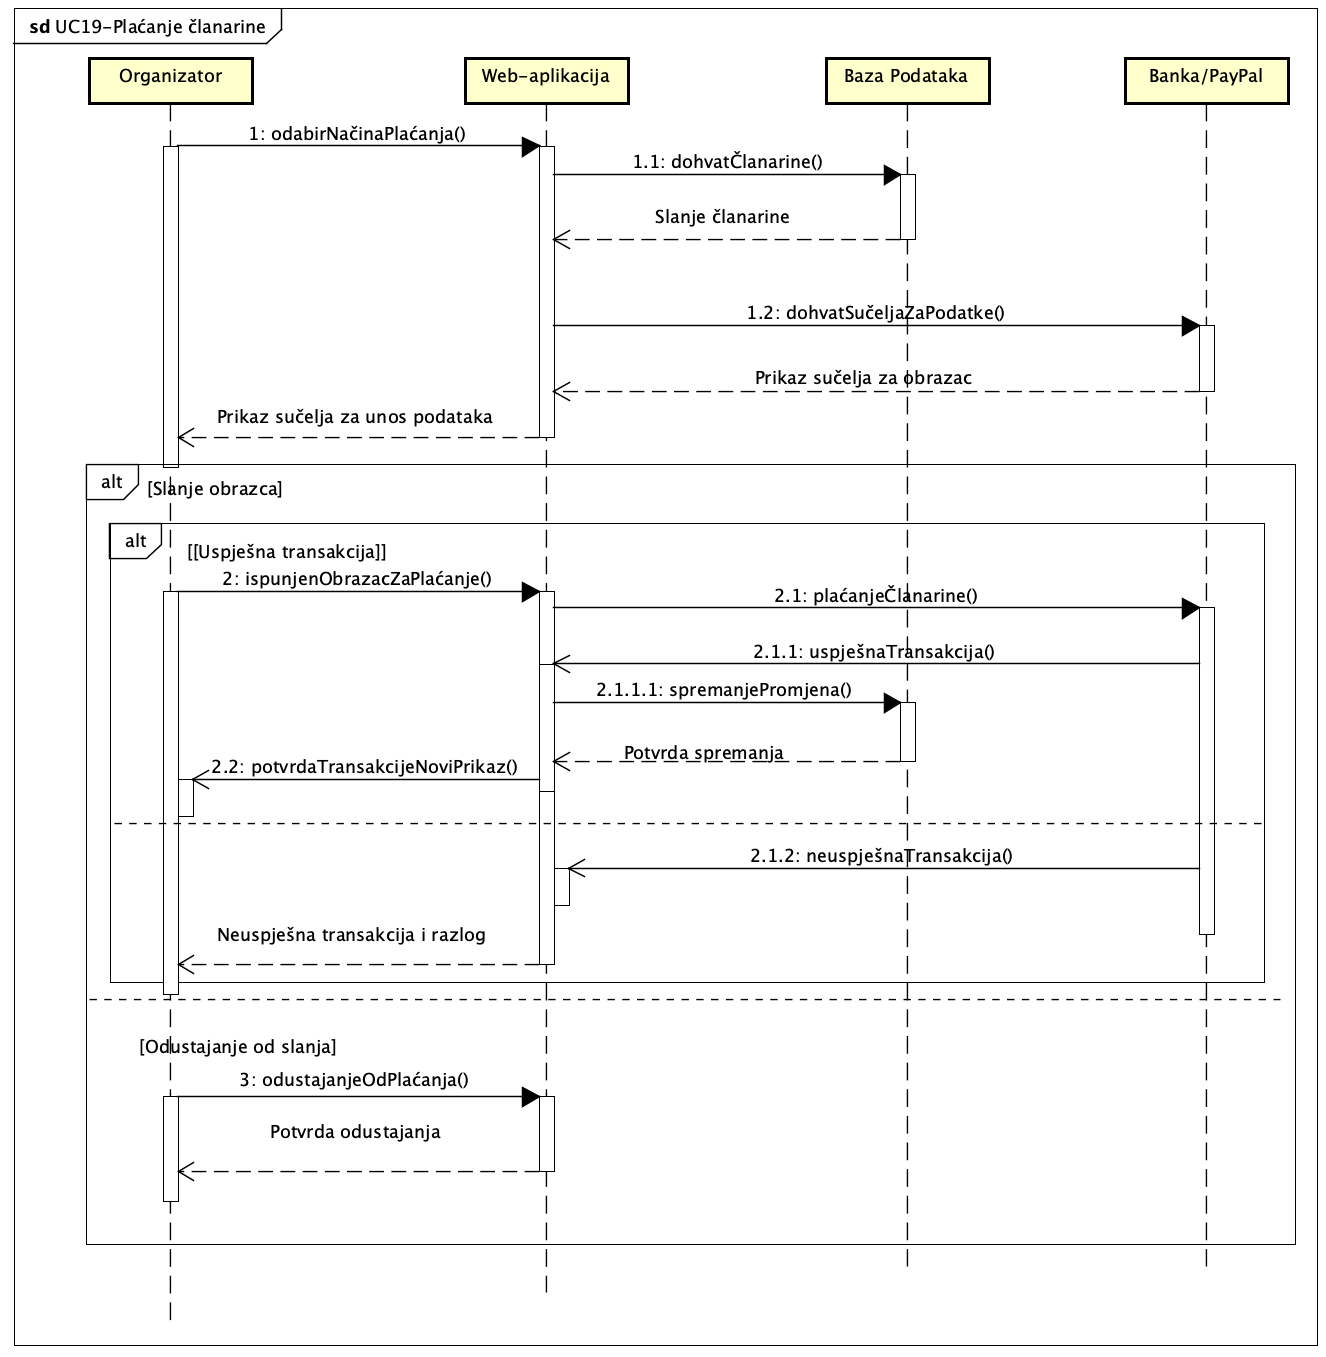
\includegraphics[scale=0.45]{dijagrami/sd-UC19-Placanje-clanarine.png} %veličina slike u odnosu na originalnu datoteku i pozicija slike
					\centering
					\caption{Sekvencijski dijagram za UC19}
					\label{fig:promjene}
				\end{figure}
				\eject		
				
		\section{Ostali zahtjevi}

			 \begin{packed_item}
			\item Sustav treba omogućiti brzo i učinkovito pregledavanje aktualnih događanja, uz minimalno vrijeme odziva aplikacije.
			\item Korisničko sučelje i sustav moraju podržavati različite vrste događanja i inicijativa, prilagođene različitim interesima zajednice.
			\item Izvršavanje dijela programa u kojem se pristupa bazi podataka ne smije trajati duže od nekoliko sekundi kako bi se osigurala brza dostupnost informacija.
			\item Sustav treba biti implementiran kao web-aplikacija koristeći suvremene tehnologije i objektno-orijentirane jezike.
			\item Neispravno korištenje korisničkog sučelja ne smije narušiti funkcionalnost i rad sustava, a sustav treba pružiti jasne upute korisnicima o načinu korištenja.
			\item Sustav treba podržavati različite načine plaćanja članarine, uključujući PayPal i kreditne kartice, te osigurati sigurnost transakcija.
			\item Veza s bazom podataka mora biti kvalitetno zaštićena, brza i otporna na vanjske greške kako bi se očuvala integritet podataka.
			\item Pristup sustavu mora biti omogućen iz javne mreže pomoću HTTPS kako bi se osigurala sigurna komunikacija između korisnika i sustava.
			\item Administratori sustava trebaju imati alate za postavljanje cijena članstva, upravljanje korisnicima i održavanje cjelokupnog sustava.
			 \end{packed_item}
			 
			 
	